\newpage
\subsubsection{Flight Report: Sensor Test}
\begin{minipage}{1\textwidth}
	\begin{flushright}
		Date: 30-05-2022\\
		Location: Hoa Phu Pump Station\\
		Coordinates: 10.9854687, 106.6186905\\
		Flight Mode: \gls{GPS}\\
		Flight Duration: 25 minutes\\\vspace{5mm}
	\end{flushright}
\end{minipage}

The goal of this flight was to fully test the second revision of the sensor package. The flight took place at the Hoa Phu Pump Station partially managed by PERNAM. A small presentation of the project goal was given before the test flight.

\begin{figure}[h]
\centering
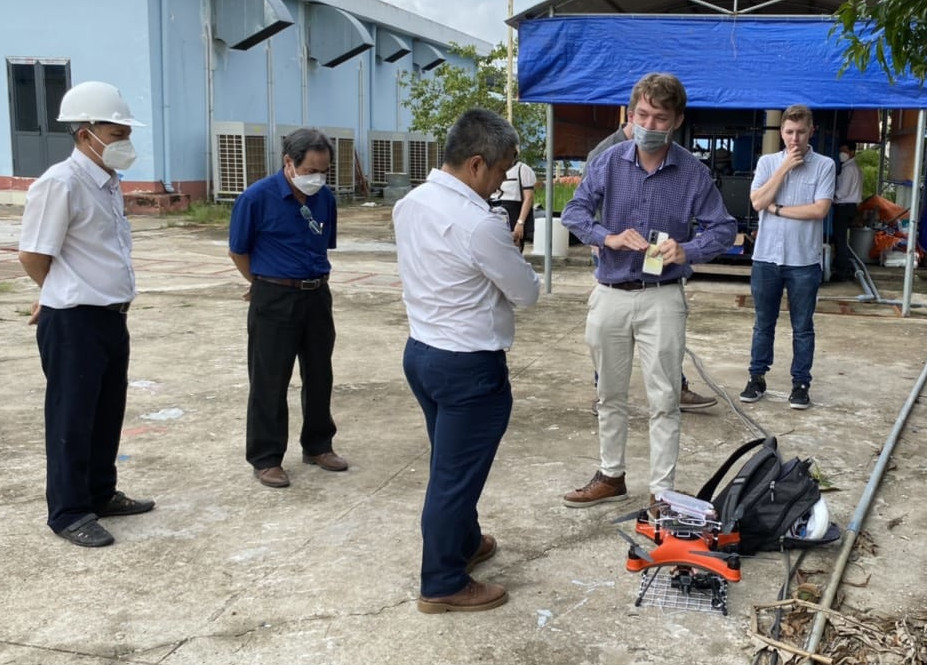
\includegraphics[scale=1.2]{080_testing/flights/32_explanation.jpg}
\caption{A small presentation about the project [own picture]}
\end{figure}

The drone seemed stable when gaining altitude. When the drone was above the water however, I noticed that it started slightly drifting away from the test site. An emergency landing had to be made, so there were several options.


One could land in the water. This was however a bit risky due to the fact that landing in the water while moving causes the drone to flip. While flipping over in the water is not an issue in normal operation of the drone, it was not clear what would happen with the sensor package. The water also had flow, so if the drone would be uncontrollable, we had to retrieve it while moving in the water.\\

I opted to bring the drone back to land so that retrieval of the drone was possible. The drone has a built in back to home function, but this did not work like intended. The drone went in the other direction, so I opted to land the drone at the other side of the land.
\newpage

\begin{figure}[h]
\centering
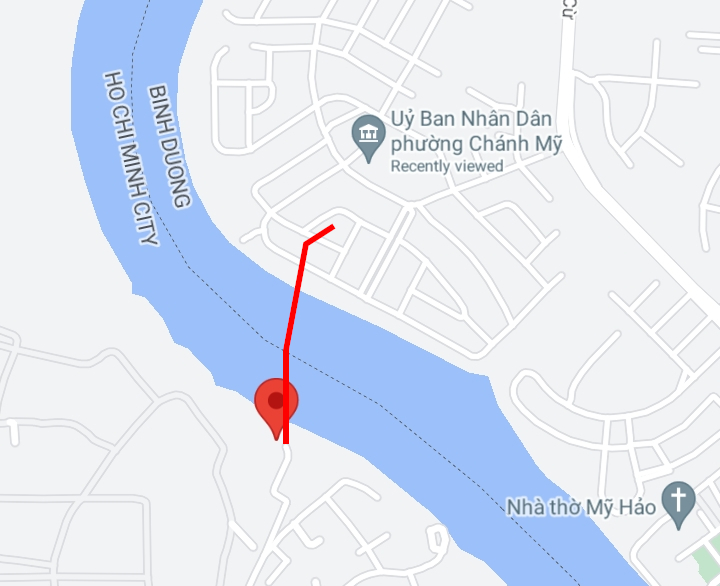
\includegraphics[scale=1.2]{080_testing/flights/31_flight.jpg}
\caption{The flight route of the drone [own picture]}
\end{figure}

This land unfortunately had high grass, so the drone did not land gracefully. Retrieving the drone was done by going to the coordinates of the remote controller. This involved a motorbike ride of 20 minutes. When I got there, the drone had 1 damaged motor and minor damage to the landing gears.

\begin{figure}[h]
\centering
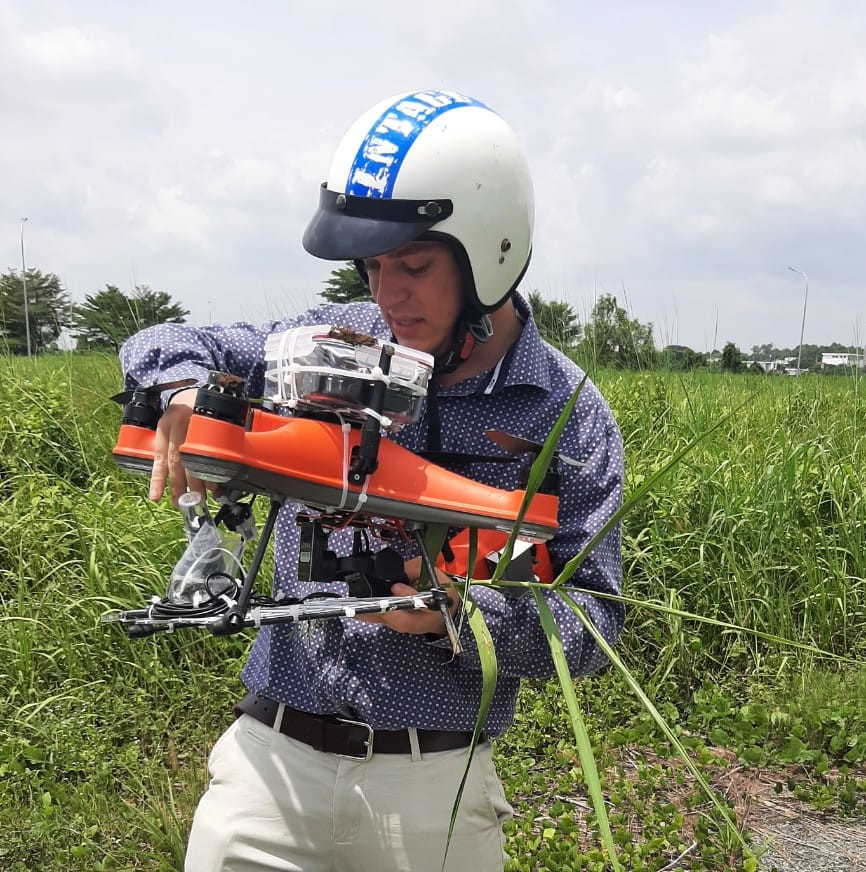
\includegraphics[scale=1]{080_testing/flights/33_afterflight.jpg}
\caption{Retrieving the drone after the crash [own picture]}
\end{figure}

\paragraph{The cause}
There could be multiple reasons why the drone reacted the way it did during the flight. The most logical explanation would be that the calibration of the drone, combined with the slight imperfections seen at the center of mass caused the drone to drift. Return-to-home may not have worked because of poor \gls{GPS} reception at the test site.

\paragraph{Improvements}
Drift would not be such an issue if the weight of the sensor enclosure would be less. Custom casing could be designed that could fit the components better.